\chapter{Euscan CLI, web interface and API}

\section{Brief history of the project}

Euscan was first started by Corentin Chary in the beginning of 2011 as a small Gentoo utility for getting upstream version information for ebuilds. Corentin announced his idea and published an initial version of the project on the \emph{gentoo-dev} mailing list \cite{euscan_announcement}.
First of all a command line interface was developed but after a few days a web interface was added. Gentoo developers liked the idea and asked for new features and gave suggestions. An announcement was posted also on the Chromium OS development mailing list to ask for feedback, as Euscan is distro-agnostic and Chromium OS is another project that uses Portage \cite{euscan_chromium}.

Euscan was also proposed by Gentoo developers for the Google Summer of Code 2012, Federico Scrinzi presented a proposal with various enhancement for the project. Federico worked during the summer and accomplished the Summer of Code goals. He kept working on the project together with Corentin until present and became officially a Gentoo developer in early 2013 to maintain Euscan and migrate it to the Gentoo infrastructure.


\section{A new approach to upstream scanning}
The power and flexibility of ebuilds allow to exploit them as a primary source of information for upstream scanning. In Debian uscan and in many other scanners the basic idea is to make the maintainer provide additional information for keeping the package up-to-date: usually an URL to scrape and a regular expression to match. This requires more effort in package creation, causes redundant information and is not always reliable.

Many packages are hosted on the same standardized service, for example almost all Python libraries are available on PyPi (\texttt{http://pypi.org}), which offers an API to get more specific and precise information about packages. As most of the packages are hosted in a few big services, using ad-hoc pieces of software to get version information allows to obtain better quality results.

Euscan exploits information included inside ebuilds to achieve this: all ebuilds provide a \texttt{SRC\textunderscore URI} variable with the URL where to get the source code. This allows to infer the best way to retrieve version information or fallback to a generic scraping in the worst cases.
It is important to remark that ebuilds do not need to provide additional information for upstream scanning, even though it is possible to do that to handle corner cases. Euscan infers all the needed information and automates the process for the maintainer.


\section{Euscan command line interface}
The command line interface is the most simple way to get information out of Euscan. Here is a basic usage example of the application:

\vspace{0.5cm}
\lstset{caption=Example of Euscan usage, label=Euscan example, numbers=none, frame=none, breaklines=true}
\begin{lstlisting}
$  euscan abiword
 * app-office/abiword-2.8.6-r2 [gentoo]

Ebuild: /usr/portage/app-office/abiword/abiword-2.8.6-r2.ebuild
Repository: gentoo
Homepage: http://www.abisource.com/
Description: Fully featured yet light and fast cross platform word processor

 * SRC_URI is 'http://www.abisource.com/downloads/abiword/2.8.6/source/abiword-2.8.6.tar.gz'
 * Scanning: http://www.abisource.com/downloads/abiword/${PV}/source/abiword-${PV}.tar.gz
 * Scanning: http://www.abisource.com/downloads/abiword
 * Scanning: http://www.abisource.com/downloads/abiword/2.9.0//source
 * Scanning: http://www.abisource.com/downloads/abiword/2.9.1//source
 * Scanning: http://www.abisource.com/downloads/abiword/2.9.2//source
 * Scanning: http://www.abisource.com/downloads/abiword/2.9.3//source
 * Scanning: http://www.abisource.com/downloads/abiword/2.9.4//source

Upstream Version: 2.9.2  http://www.abisource.com/downloads/abiword/2.9.2//source/abiword-2.9.2.tar.gz
Upstream Version: 2.9.3  http://www.abisource.com/downloads/abiword/2.9.3//source/abiword-2.9.3.tar.gz
Upstream Version: 2.9.0  http://www.abisource.com/downloads/abiword/2.9.0//source/abiword-2.9.0.tar.gz
Upstream Version: 2.9.1  http://www.abisource.com/downloads/abiword/2.9.1//source/abiword-2.9.1.tar.gz
Upstream Version: 2.9.4  http://www.abisource.com/downloads/abiword/2.9.4//source/abiword-2.9.4.tar.gz
\end{lstlisting}
\vspace{0.5cm}

It is possible to customize the behavior of Euscan by using command line parameters. The following list describes the most noteworthy ones:
\begin{itemize}
\item \emph{format}: Euscan can output information in a machine readable format, in order to make it easy to develop other applications that exploit its functionalities. Currently JSON and XML output are supported.
\item \emph{ignore-pre-release} and \emph{ignore-pre-release-if-stable}: these options allow to ignore pre-releases (alpha, beta, rc, ...) if the user is interested only in stable updates. It can happen that not stable versions are not considered valuable and do not deserve a version bump. The first option ignores all pre-releases while the latter ignores them only if the latest package version is a stable release.
\item \emph{no-handlers}: disables some specific handlers. Handlers are specialized methods to detect upstream versions with a better accuracy (see section \ref{sec:handlers}). 
\end{itemize}


\section{Euscan web interface}
Euscan is primarily intended to be used through a web interface. Euscanwww is a \emph{Django} (\texttt{http://djangoproject.org}) application that offers a plethora of functionalities to ease the maintenance work and show insightful information about the status of the Portage tree.

\subsection{Ebuild browsing}
The very basic functionality of the web interface is an overview of all the ebuilds available in the Portage tree and major overlays. It is possible to browse packages per category or per overlay, but also per herd or per maintainer. These latter features are useful for maintainers, for getting a summary of the ebuilds they are entitled to.

This interface offers per package information about available versions in Portage or overlays, as well as upstream ones.
For obtaining information about the status of the Portage tree and the overlays, a scan process is started periodically. For performance reasons the whole data is replicated and denormalized into a relational database.

For each group of packages it is possible to sort and filter the results using different metrics:

\begin{itemize}
\item last version in Portage;
\item last version in any of the overlays;
\item last upstream version not in Portage;
\item number of Portage versions;
\item number of overlays versions;
\item number of upstream versions not in Portage;
\item ratio of Portage or overlay versions over total number of versions.
\end{itemize}

By selecting a package it is possible to get a detailed view of its properties: name, homepage, maintainers, herds, ebuild's content, ebuild's metadata, Portage versions, overlays versions, upstream versions, a brief history of its versions and the log of the last Euscan scan.


\subsection{User dashboard}
Euscanwww provides a registration system to let users register, login and use a platform customized to their needs. An authenticated user is allowed to access to additional features:

\begin{itemize}
\item Request package refresh: A registered user can request a package scanning, to be sure that a specific package has fresh information. When this process is requested the job is sent to a queue. It asynchronously launches a task that scans the Portage tree and overlays and then upstream. In order to prevent ungraceful system usage and abuse the queue performs a maximum of a task per minute.

\item Watch items: It is possible to watch a package or an entire category, herd or maintainer's package list by clicking on a "star" icon in the detail page of every item.

\item Dashboard: A summary of the watched packages with an overview of the number of upstream versions detected. From the dashboard is also possible to customize the RSS feed default preferences (see \ref{subsec:rss}) and the mail settings.

\item User RSS feed: A custom feed with only news from watched items.

\item Custom emails: every registered user can receive an email with updates about the items he is watching. It is possible to get a digest email every week, every month or after every scan. As for CLI and RSS feeds, it is possible to ignore pre-releases.
\end{itemize}

These features make Euscan highly customizable and flexible, in order to be suitable for any developer. Moreover the possibility of watching the maintainer's packages allows a very quick bootstrap for new developers that want to start being notified about upstream changes.


\subsection{RSS feeds}
\label{subsec:rss}

In order to allow maintainers to stay up-to-date with Euscan results, the community suggested to offer an RSS feed with package information and news. The web interface offers various level of detail and customization for these feeds:
\begin{itemize}
\item Global: feed with both upstream and Portage new versions of the whole ebuild ecosystem.

\item Per category: feed with information about all packages in the given category.

\item Per herd: feed with information about all packages that belong to the given herd.

\item Per maintainer: feed with information about all packages that belong to the given maintainer.

\item Per package: feed with information about a specific package.

\item Per user: customized feed for packages watched by the current user.
\end{itemize}

\vspace{0.5cm}

RSS options (settable using HTTP GET parameters):
\begin{itemize}
\item portage\textunderscore info: show Portage tree changes;
\item upstream\textunderscore info: show upstream versions;
\item ignore\textunderscore pre: ignore pre-releases (i.e.: alpha, beta, rc, \ldots);
\item ignore\textunderscore pre\textunderscore if \textunderscore stable: ignore pre-releases only if Portage offers a stable version.
\end{itemize}


This level of granularity and customization allows to use Euscan not only as an upstream scanner, but also for getting other useful information about how the Portage tree is evolving. Moreover the possibility to ignore certain types of upstream versions allows to exclude false positives, basing on the maintainer's policies.


\subsection{REST API}
Euscan provides a REST API to query the service. At the moment it does not provide a rich set of features: it is mostly meant to give statistics about the status of the Portage tree and upstream versions.
Improving the API and adding more functionalities is one of the next steps for the future.


\subsection{Statistics}
For the purpose of giving a clear and insightful overview of the status of the Portage tree and its health, Euscan offers different kind of statistics.
For instance, for the whole system or for every category, herd and maintainer it is possible to get quantitative information about how many packages are updated (either in Gentoo or in some overlay) or are out-of-date. Historical information is available in order to detect improvement or regression in the management of the ebuilds.
Graphs are generated using \emph{rrdtool} (\texttt{http://oss.oetiker.ch/rrdtool/}) because of its high performance and easy integrability.
It is also possible to have an overview of the methodologies used to detect upstream versions, the average confidence that Euscan assigned to its work (see \ref{sec:handlers}) and to get a glance of the configuration of the Euscan web instance.

\begin{figure}[h!]
  \centering
    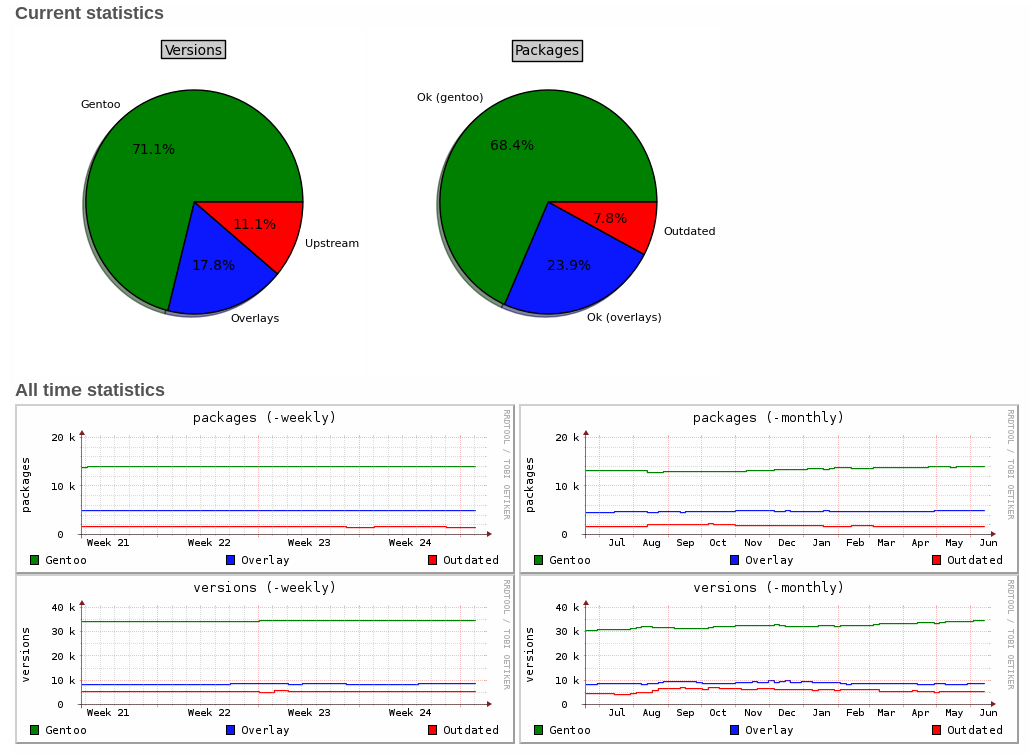
\includegraphics[width=13.5cm,natwidth=1030,natheight=754]{img/statistics.png}
  \caption{Euscan global statistics}
\end{figure}


\subsection{Tasks}
Many asynchronous tasks are provided by the Euscan web interface for scanning the Portage tree, detecting upstream versions and, more generally, updating the local database with fresh data.
The handling of these operations is entrusted to \emph{Celery} (\texttt{http://celeryproject.org/}) and distributed to different workers using \emph{RabbitMQ} (\texttt{http://rabbitmq.com/}).

Some examples of the available tasks are the following:
\begin{itemize}
\item update\textunderscore portage\textunderscore trees: Synchronizes the Portage tree and all the overlays to the latest release. This operation is usually performed before an upstream scanning process.

\item scan\textunderscore portage: uses \emph{eix} (\texttt{http://eix.berlios.de/}), a tool for Gentoo for quick searching in the Portage tree. Eix offers good performance and it can output machine readable data in the XML format. The XML stream is parsed on the fly, newly found packages and versions are used to populate the Euscan database.

\item scan\textunderscore metadata: extracts metadata for every package found in Portage using the \emph{Gentoolkit} (\texttt{http://www.gentoo.org/doc/en/gentoolkit.xml}) Python API. An example of metadata is herd's and maintainer's information.

\item scan\textunderscore upstream: uses the Euscan Python API to detect new upstream versions. 

\item regen\textunderscore rrds: Regenerates statistics graphs. For performance reasons all the graphs displayed in the Euscan web interface are not computed on the fly but are generated after a scan process and then are cached.

\item update\textunderscore counters: Updates all cached attributes. For performance reasons some computationally expensive pieces of information are calculated only once and then are stored (e.g.: the number of upstream versions per package, last Portage version for each package or being or not the latest version).
\end{itemize}


\subsection{Admin panel}
The Django admin panel has been customized for Euscan purposes. Apart from managing all Euscan data, using this interface it is also possible to launch scanning and utility tasks or schedule them periodically.


\subsection{Technical issues}
\subsubsection{Long running asynchronous tasks}
All background tasks are handled by Celery with different workers for parallelization. As Euscan needs to handle more than 20000 packages and perform tasks on each package, these tasks are crucial for the reliability of the platform. During the development, this part of the software was the one that revealed more issues and bugs because of the difficulty of testing all the functionalities in every edge case. Before the GSoC 2012, Euscan used a Bash script and GNU Parallel (\texttt{https://www.gnu.org/software/parallel/}) but this was not manageable from the web UI as it was running with \emph{cron} and was not so performant (it required the call of the Python interpreter for every package).

With Celery it is possible to easily scale by adding more and more workers (even on different machines) and manage everything from the Django admin panel or using a Python API.
A big issue was the synchronization of the different processes because there is the need of sequentiality (first of all get data from the ebuilds, then scan upstream) and avoidance of deadlocks. As the number of workers is limited, if a task hangs for example because of network issues, that worker becomes unavailable; if all workers become unavailable the whole scan process is stalled. To resolve this problems the code was tweaked to handle errors and Celery tools like chords and grouping are used for synchronization \cite{celery_doc}.

Various tests were made in order to find a good configuration for achieving reasonable performance. The results are as follows:
\begin{itemize}
\item For Portage and metadata scanning the is no a priori knowledge of the all the available packages, as new ones can be released. For this reason it is not possible to run a subtask for getting information about a single package or a group of them. Moreover, most of the time required to get this kind of information is spent by eix or gentoolkit: Euscan code just retrieves eix results and stores them into its database after a simple parsing of the given data. A good solution that was even used in production for some time was to use a single task to perform the work for the whole ebuild tree. This approach however did not offer any kind of parallelization, making the process reliable but not fast. The current implementation divides the scanning load by category: there are 153 categories in Portage, each task scans one of them.

\item For upstream scanning and other network dependent tasks (like sending emails) a different approach was used. As each single task is slow and can possibly crash because of network issues it is a good choice to isolate them. For this purpose Celery offers subtasks, independent tasks that belong to a higher class task that manages them. Subtasks can run in parallel and then be joined to their parent task.
For upstream scanning there is a priori knowledge of the packages to scan, so it is possible to create a task that deals with a group of packages, where the scanning process for each package is performed by a subtask. The same applies for email sending.
This approach is better than launching many "real" tasks because each one of them is sent to Celery using RabbitMQ and sending tens of thousands of messages to the queue creates too much overhead.
\end{itemize}

\subsubsection{Data model design and performance}
Creating a performant data model for the ebuild tree requires some effort and shrewdness: the packages available in Gentoo are around 20000 and there are more than 30000 versions associated to them. Moreover each package has a relation with a maintainer or a herd (note that these are many-to-many relations). With this kind of data performing joins can be very expensive and for offering interesting information to Euscan users there is the need of computing the results of many aggregation functions. A very common query is \emph{"give me the number of packages for each maintainer that have at least a new upstream version"}: this operation requires a join between the table of packages, versions, packages-maintainers (table that handles the many to many relation) and maintainers, then there is the need to apply grouping and aggregations.

To solve this issues, commonly used operations are computed after each scan process and its result is cached. This approach is possible because data is changing only after a scan process. Furthermore, for faster queries through the Django ORM, \emph{select\textunderscore related} and \emph{prefetch\textunderscore related} features are used extensively \cite{django_orm}.

\section{Euscan Python API}
Euscan is also a Python module with a wide set of utilities for scanning upstream. In fact, the CLI and the Web interface share the same common code and are built upon the Euscan Python API. Nothing prevents another application to exploit the Euscan functionalities for its own purpose.
